\documentclass[12pt,a4paper]{article}

\usepackage[utf8]{inputenc}
\usepackage[greek,english]{babel}
\usepackage{alphabeta} 

\usepackage[pdftex]{graphicx}
\usepackage[top=1in, bottom=1in, left=1in, right=1in]{geometry}

\linespread{1.06}
\setlength{\parskip}{8pt plus2pt minus2pt}

\widowpenalty 10000
\clubpenalty 10000

\newcommand{\eat}[1]{}
\newcommand{\HRule}{\rule{\linewidth}{0.5mm}}

\usepackage[official]{eurosym}
\usepackage{enumitem}
\setlist{nolistsep,noitemsep}
\usepackage[hidelinks]{hyperref}
\usepackage{cite}
\usepackage{lipsum}
\hypersetup{
    colorlinks=true,
    linkcolor=blue,
    filecolor=magenta,      
    urlcolor=blue,
    pdftitle={Overleaf Example},
    pdfpagemode=FullScreen,
    }


\begin{document}

%===========================================================
\begin{titlepage}
\begin{center}

% Top 

\includegraphics[width=0.95\textwidth]{images/Trinity_Main_Logo.jpeg}~\\[2cm]


% Title
\HRule \\[0.4cm]
{ \LARGE 
  \textbf{Biography of a Software Engineer}\\[0.4cm]
  \emph{Jawed Karim, Co-Founder of YouTube}\\[0.4cm]
}
\HRule \\[1.5cm]

\bigbreak

\vskip 1in

% Author
{ \large
  Prathamesh Sai \\[0.1cm]
  3rd year Integrated Computer Science\\[0.1cm]
  Student ID: 19314123\\[0.1cm]
}

\vfill

%\textsc{\Large Cyprus University of Technology}\\[0.4cm]
\textsc{\large School of Computer Science and Statistics,\\Trinity College Dublin}\\[0.4cm]


% Bottom

 
\end{center}
\end{titlepage}



\newpage



%===========================================================

\newpage
\setcounter{page}{1}

%===========================================================
%===========================================================
\section{Introduction}\label{sec:intro}
Jawed Karim was born on the 28th of October 1979 in a town in Central Germany called Merseburg. His father Naimul Karim was a researcher from Bangladesh and his mother Christine Karim was a German research professor of biochemistry at the University of Minnesota. At a very young age, his family had to leave communist East Germany and immigrate to West Germany where he spent most of his childhood. At the age of 12, he moved to Saint Paul in Minnesota. It was clear that Jawed was interested in Computer Science and Software Engineering from a young age, so he decided to study Computer Science at the University of Illinois Urbana-Champaign. However, Jawed ended up leaving campus before graduating to join PayPal as one of it's first employees. He didn't drop out, but continued his education remotely while working at PayPal. While working there in 2002, he met Steve Chen and Chad Hurley who would help him become the co-founder of a soon-to-be billion dollar company.

\section{The reason behind creating YouTube}\label{sec:lit-rev}
Jawed was frustrated by the non-existence of video clips of the Super Bowl XXXVIII and the Indian Ocean earthquake and tsunami in 2004. This led to the idea of creating a video sharing platform that people could use to upload videos to share with their friends online. After discussing the idea with Steve and Chad, the YouTube domain name was activated on the 14th of February 2005, with the co-founders developing the website over the next few months. Jawed then made the first ever YouTube Channel "jawed" on the 23rd of April 2005 and uploaded the website's first video called "Me at the zoo" recorded by his high school friend Yakov Lapitsky. The video is currently at almost 200 million views.

\begin{center}
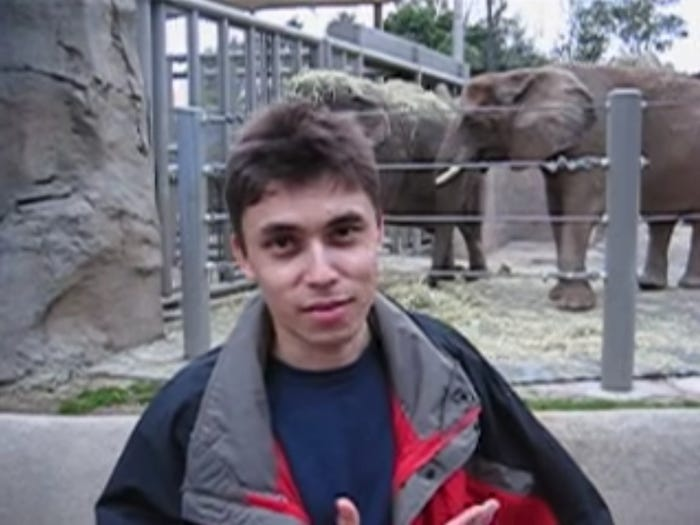
\includegraphics[scale=0.4]{images/Jawed.jpeg}
\end{center}

\section{Getting funding for YouTube}\label{sec:meth}
It was evident to Jawed that without funding, YouTube would not reach anywhere near it's full potential. It needed some sort of funding for it to be a successful business. Therefore the company started as a venture capital-funded technology startup. This allowed the co-founders to gather funding to get YouTube on it's feet. The co-founders soon ended up with almost \$20 million dollars in funding from Sequoia Capital and Artis Capital Management. This funding was crucial to YouTube's success, as it not only helped the company financially, but it also gave people a reason to believe that it would be a successful avenue to pursue. 

\section{Going back to education}\label{sec:res}
After launching YouTube, Jawed still had the desire to complete his studies. Although he knew YouTube would be successful if we worked on it full-time, he went on to subsequently join Stanford University as a graduate student after finishing his undergraduate studies remotely. He had a love for education, and even though he knew he could potentially make more money through YouTube, he decided to not work as an employee at YouTube, but rather as an informal advisor. The decision to focus on formal education instead of working on YouTube meant that he took a lower share in the company compared to the other co-founders. While he left, YouTube started gaining traction and even got it's first video with one million views within it's first year — A video by Nike featuring Ronaldinho receiving his pair of "Golden Boots".

\begin{center}
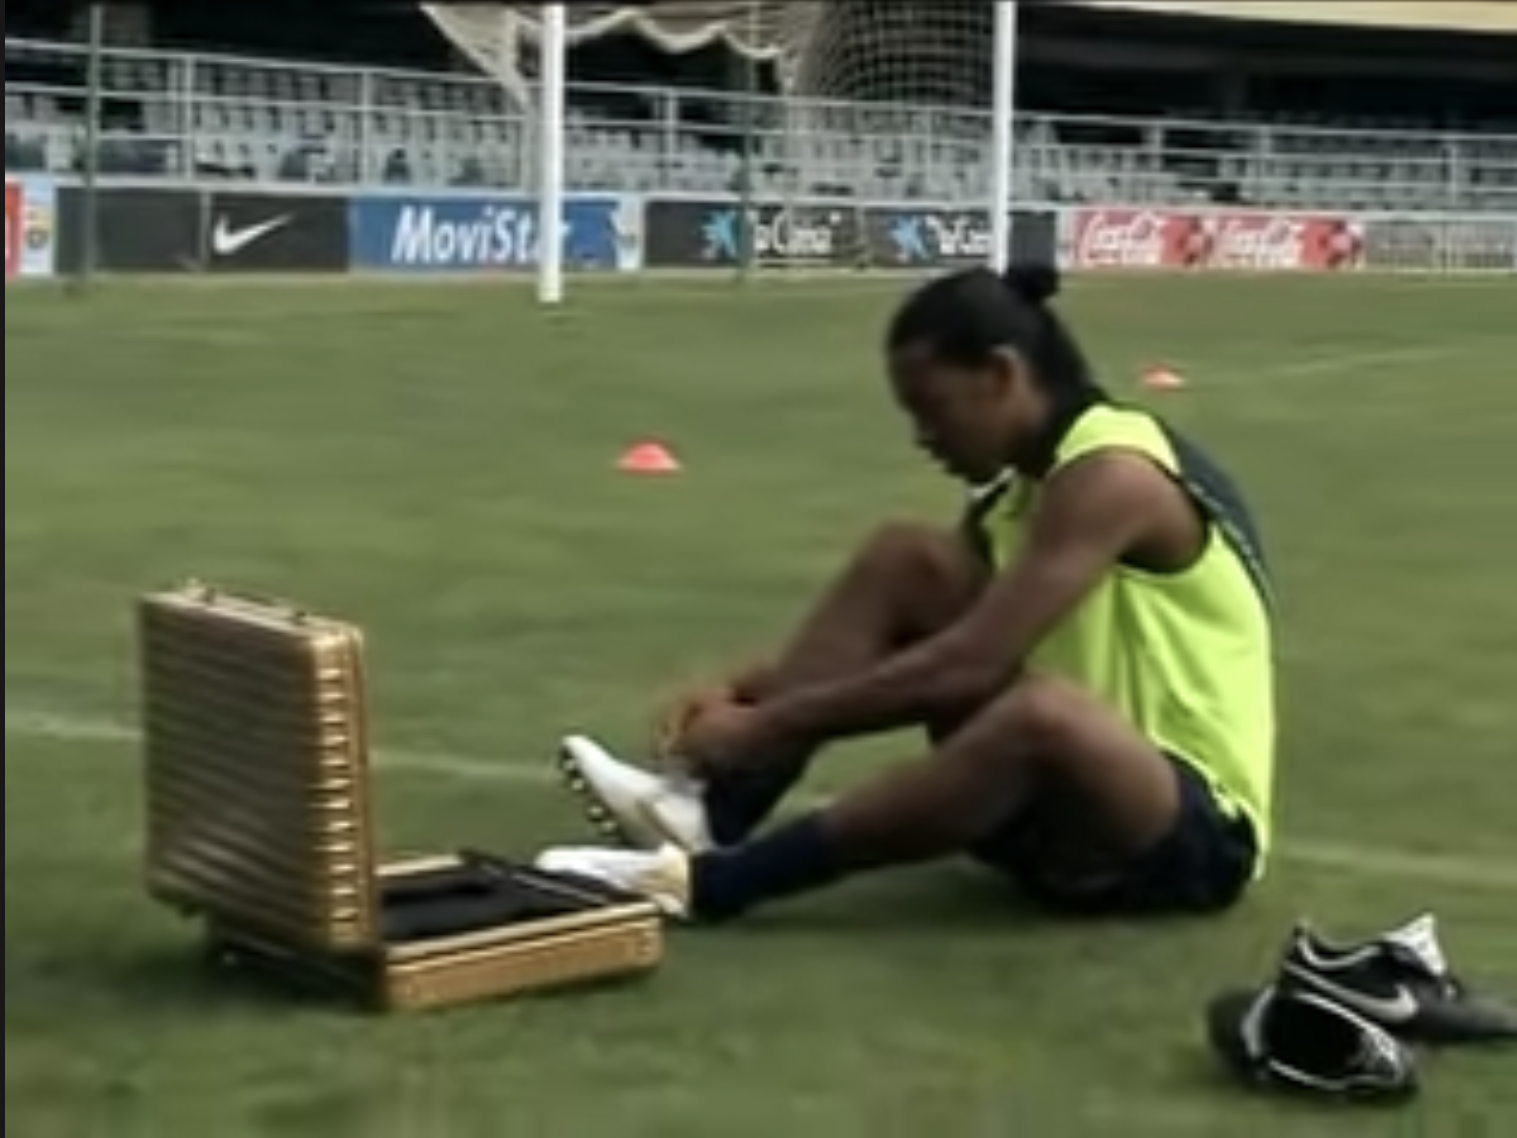
\includegraphics[scale=0.4]{images/Ronaldinho.png}
\end{center}

\section{Life after selling YouTube}\label{sec:res2}
As YouTube grew in popularity, it was evident that the co-founders did everything they could to grow YouTube to the point it was at. However, they felt that they needed to let an experienced leader in the field buy the company for the right price, to bring YouTube to the next level. Many big companies such as Microsoft, Viacom, and Yahoo were interested in buying YouTube, but YouTube's current CEO Susan Wojcicki's who worked at Google loved the concept of the video sharing platform and decided to take charge of acquiring it. In 2006, YouTube was sold to Google for \$1.65 billion dollars. Since then, the three co-founders have been away from the spotlight, investing their new found wealth into exciting ideas and experimenting with different business ventures. For example, Jawed invested in the initial seed round of Airbnb Inc, becoming one of the initial investors of the company valuated at over 100 billion after their initial IPO.
\begin{center}

\includegraphics[scale=0.2]{images/GoogleYoutubeLogo.png}
\end{center}
\section{How he shaped my view of Software Engineering}\label{sec:res3}
I chose Jawed Karim because of his skill of identifying a niche, and using software engineering practices to build something so crucial to people around the world. As cliché as it sounds, Jawed never developed YouTube with the desire for it to be used by millions of people. He simply solved a personal problem he was facing, later realising that it could be used by other people. This is how many of the biggest companies started, and it's one of the reasons why I wanted to study Computer Science in the first place. His eye for spotting potential, and using his knowledge to develop it into something greater is something I look up to.

\bibliographystyle{ieeetr}
\bibliography{refs}
• \href{https://real-leaders.com/jawed-karim-co-founder-youtube/}{\underline{An article explaining key events in Jawed's life.}}
\newline
• \href{https://en.wikipedia.org/wiki/Jawed_Karim}{\underline{Jawed's dedicated Wikipedia page showcasing his life events.}}
\newline
• \href{https://www.thequint.com/tech-and-auto/tech-news/youtube-turns-14-youtube-founders-steve-chen-jawed-karim-chad-hurley-2019#read-more}{\underline{An article explaining some background about the founders of YouTube.}}
\newline
• \href{https://youtu.be/jNQXAC9IVRw}{\underline{The first video on YouTube.}}
\newline
• \href{https://youtu.be/cTY4Yo2SR2o}{\underline{The first video on YouTube to get one million views.}}
\newline
• \href{https://valiantceo.com/jawed-karim/}{\underline{An article explaining Jawed's achievements.}}
\newline
• \href{https://www.vizaca.com/jawed-karim-entrepreneur/}{\underline{An article version of a biography of Jawed Karim.}}
\newline
• \href{https://handwiki.org/wiki/Biography:Jawed_Karim}{\underline{A wiki page about Jawed's life.}}
\newline

\end{document} 
